\chapter{Vertical Manual Screen}
\section{Overview}The \textbf{Vertical Manual} screen (Figure 4.1) is the \textit{Hand} mode operation screen for control of the \textbf{Vertical} axis of the saw. On this screen are the controls to move the \textbf{Vertical} axis through it's travel limits as well as \textbf{Home} the axis. There is also an \textbf{Indicator} for \textbf{Home} position indication, and a display area for position feedback of the axis. The \textbf{Vertical Manual} screen is a sub-screen of the main \textbf{Manual} screen. As this is the case navigation is capable back to the main \textbf{Manual} screen, the \textbf{Cut Program} screen, and both the \textbf{Cross Travel} and \textbf{Long} manual screens. As always, the \textbf{Menu} FKey will return the Operator to the \textbf{Main} screen.
\begin{figure}
	\centering
	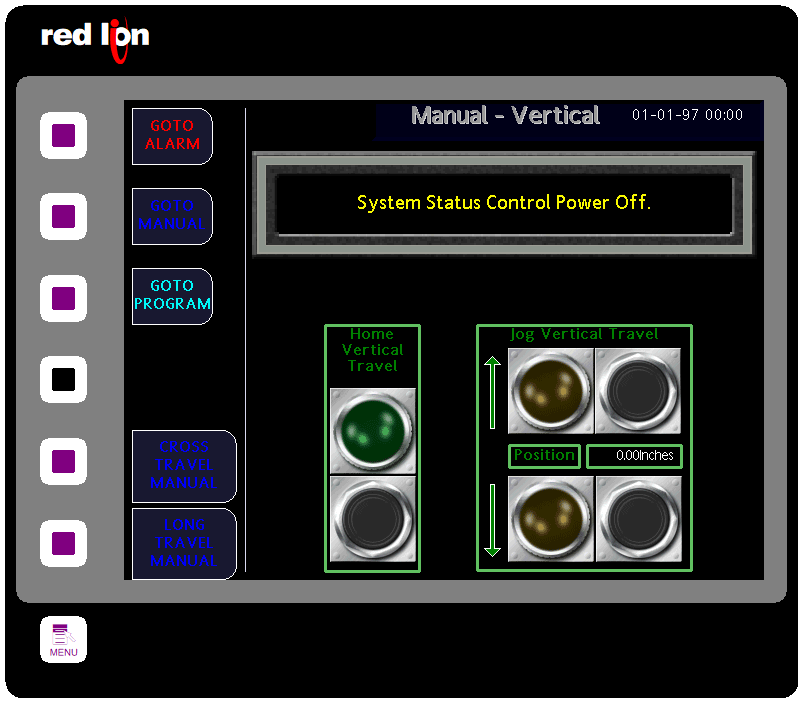
\includegraphics[width=0.5\linewidth]{screen-captures/vert-manual}
	\caption{Vertical Manual Screen}
	\label{fig:manual-vertical-screen}
\end{figure}
\pagebreak
\nopagebreak
\section{Details}The \textbf{Vertical Manual} screen details are divided into the following categories ...
\begin{list}{$\diamond$}{}
	\item \textbf{Screen Navigation}
	\item \textbf{Vertical Home}
	\item \textbf{Vertical Travel}
\end{list}
\begin{figure}
	\centering
	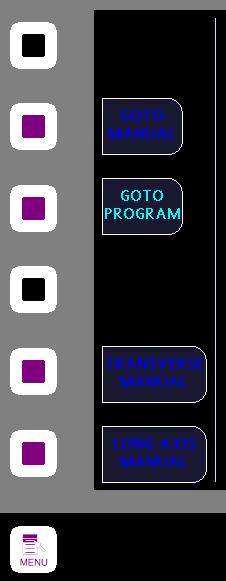
\includegraphics[width=0.2\linewidth]{screen-captures/vert-manual-nav}
	\caption{Vertical Manual Screen Navigation}
	\label{fig:manual-vertical-screen-nav}
\end{figure}
\subsection{Screen Navigation}Is performed by using the programmable Function Keys (FKeys) located down the left hand side of the OI Terminal (refer to Figure 4.2). The Operator may navigate to the following screens ...
\begin{list}{$\diamond$}{}
	\item \textbf{GOTO MANUAL} Navigate to Manual Screen.
	\item \textbf{GOTO PROGRAM} Navigate to Cut Program Screen.
	\item \textbf{CROSS TRAVEL MANUAL} Navigate to Cross Travel Manual Control Screen.
	\item \textbf{LONG AXIS MANUAL} Navigate to the Long Axis Manual Control Screen.
\end{list}
\paragraph*{\textbf{\LARGE \textcolor{blue}{i}}}
The Menu Key located on the terminal at the lower left below the FKey's, will return the Operator to the Main Screen, from all other screens.\\
\begin{minipage}{4cm}
	\begin{picture}(20,70)
	
\includegraphics[width=.5\linewidth]{screen-captures/menu}
	\end{picture}
\end{minipage}\begin{minipage}[]{11cm}
	\paragraph{\textbf{\LARGE \textcolor{blue}{i}}} The Menu Key is pictured as it looks on the Terminal.
\end{minipage}
\pagebreak
\nopagebreak
\begin{figure}
	\centering
	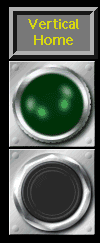
\includegraphics[width=.2\linewidth]{screen-captures/vert-manual-home}
	\caption{Vertical Manual Home Function}
	\label{fig:vert-manual-home}
\end{figure}
\subsection{Vertical Home} Function is the stand alone homing routine for the \textbf{Vertical} axis. There is a \textbf{Control} pushbutton to initiate the homing function and an \textbf{Indicator} pilot light to indicate when the \textbf{Vertical} axis is in the \textbf{Home} position and has completed a homing function. On the saw the \textbf{Vertical} axis has it's \textbf{Home} position at the raised travel limit sensor. In fact the raised travel limit proximity sensor is the \textbf{Home} proximity sensor. A homing function will cause the axis to move in either direction depending upon the state of the \textbf{Home} sensor. If the \textbf{Home} sensor is off, the \textbf{Home} function will command the \textbf{Vertical} axis to raise up to the point the sensor comes on. The axis will then stop, reverse back off of the sensor, then creep back up until the sensor triggers again. By homing in this fashion, the repeatability of the \textbf{Vertical} axis is more consistent than homing until the sensor is triggered then stopping would be.
\\
\\
\\
\\
\\
\\
\\
\\
\pagebreak
\nopagebreak
\begin{figure}
	\centering
	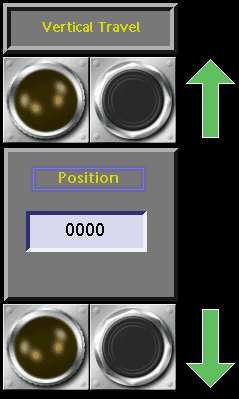
\includegraphics[width=.2\linewidth]{screen-captures/vert-manual-command}
	\caption{Vertical Manual Travel}
	\label{fig:vert-manual-command}
\end{figure}
\subsection{Vertical Travel} Figure 4.4 above shows the \textbf{Vertical Travel} function. The function is made up of a pushbutton to command \textbf{Vertical Travel Raise} with a corresponding \textbf{Indicator} pilot light that indicates motion commanded but not complete. There is also a corresponding \textbf{Vertical Travel Lower} pushbutton and \textbf{Indicator}. Finally, there is a position feedback display area which shows the current axis position in inches. This function is available in \textit{Hand} mode and is intended for use by the Operator during Machine Setup and Maintenance activities. 
\paragraph*{\textbf{\LARGE \textcolor{blue}{i}}}The position feedback should be considered invalid if the axis has not been homed yet, since the position encoder is an incremental encoder and does not retain position information on a power cycle. Therefore it is required to reference the axis feedback to zero on successful homing completion, in order to ensure positional accuracy and repeatability.
\\
\\
\pagebreak
\nopagebreak
